\section{Lösungsansätze} \label{sec:Loesungsansaetze}

Bereits im Abschnitt \ref{sec:AuswahlMetaheuristischenAlgorithmen}  wurden Metaheuristiken und andere Lösungsansätze selektiert, um Zeitpläne für das \ac{mrcpsp} zu finden. Als abstrakte Anlaufstelle für die Lösungsverfahren dient das Interface \lstinline|Solver|, welches eine Methode \lstinline|algorithm(...)| vorsieht. Dieses wird parametrisiert über ein \lstinline|Benchmark|-Objekt, die Anzahl an Iterationen, eine Robustheitsfunktion und eine feste Anfangsliste von Aktivitäten- und Modi, welche wiederum relevant für die reaktiven Verfahren sind. Aufgerufen wird die Methode über die einzelnen Experimente. Die konkreten Lösungsansätze implementieren diese Methode gemäß des eigentlichen Algorithmus. Für den fairen Vergleich der Algorithmen werden die Iterationen als ein Zähler von erzeugten Aktivitäts- und Moduslisten betrachtet. Das Erzeugen eines Tupels erhöht die durchlaufene Iterationen um eins. Bei einer Nachbarschaft aus fünf Elementen dementsprechend um fünf. \\

Das UML-Klassendiagramm aus Abbildung \ref{img:mrcpsp_framework_solver} zeigt das Zusammenspiel der Lösungsverfahren genauer auf. Alle aus Abschnitt \ref{sec:AuswahlMetaheuristischenAlgorithmen} selektierten Lösungsansätze werden über eine eigene Klasse repräsentiert, welche das Interface \lstinline|Solver| implementieren. Diese erzeugen über die jeweiligen Algorithmen die Aktivitäts- und Moduslisten, um so Zeitpläne über den \lstinline|SchedulerService| zu erzeugen. Insbesondere für die initialen Lösungen nutzen die Metaheuristiken den \lstinline|HeuristicDirector|, um so machbare oder sogar gute Lösungen zunächst heuristisch zu generieren. Insbesondere der \lstinline|GeneticAlgorithm| nutzt für die initiale Population unterschiedliche Prioritäts- und Selektionsregeln. \\

Ebenfalls im Abschnitt \ref{sec:AuswahlMetaheuristischenAlgorithmen} wurde eine gemeinsame Nachbarschaftsfunktion für sowohl Hill Climbing, Tabu Search als auch Simulated Annealing festgelegt. Die Funktionsweise der implementierten Nachbarschaftsfunktion $\Tilde{N}(s)$ ist in Abbildung \ref{img:implementation_neighbourhood} illustriert. Für einen zu betrachtenden Zeitplan $s$ werden stets zwei Zeitpläne in der Nachbarschaft hinzugefügt, welche eine identische Aktivitätsliste zum Basisplan aufweisen. Dennoch wird abweichend zum Basisplan ein Modus innerhalb der Modusliste umgedreht. Alle vom Basisplan aus gültigen Aktivitätsswaps werden ebenfalls einschließlich eines Moduslistenelement-Flip in der Nachbarschaft hinzugefügt. \\

\begin{figure}[H]
    \centering
    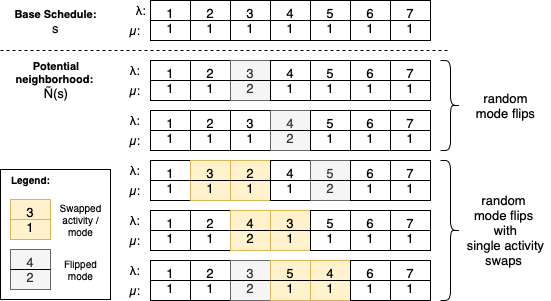
\includegraphics[width=0.84\linewidth]{assets/img/04_Umsetzung/MRCPSPNeighhbourhood.drawio.png}
    \caption{Funktionsweise der implementierten Nachbarschaftsfunktion anhand eines Beispiels für den Projektplan aus Abbildung \ref{img:visualization_projectplan}} 
    \label{img:implementation_neighbourhood}
    \source{Eigene Darstellung}
\end{figure}

In den folgenden Unterabschnitten werden die implementierten Lösungsansätze für das \ac{mrcpsp} erläutert. Zunächst wird im Abschnitt \ref{subsec:Naiv_Random} die Umsetzung der Erstellung von zufälligen Lösungen vorgestellt. Im Folgeabschnitt \ref{subsec:Hill_Climbing} wird der Hill Climbing-Algorithmus behandelt. Die Tabu Suche wird in Ausschnitt \ref{subsec:MetaheuristischeAlgorithmen_TabuSearch} erläutert, den Simulated Annealing-Algorithmus in Abschnitt \ref{subsec:MetaheuristischeAlgorithmen_SimulatedAnnealing}. Zuletzt gilt es den umgesetzten genetischen Algorithmus im Abschnitt \ref{subsec:MetaheuristischeAlgorithmen_EvolutionaereAlgorithmen} vorzustellen.

\subsection{Zufällige Lösungen} \label{subsec:Naiv_Random}

Den einfachsten Lösungsansatz stellt das Generieren von zufälligen Lösungen dar. Der \lstinline|RandomSolver| generiert mit Hilfe des \ac{ssgs} und dem \lstinline|HeuristisDirector| zunächst syntaktisch korrekte Zeitpläne. Hierbei werden als Prioritäts- und Selektionsregeln die Klassen \lstinline|RandomActvitiyHeuristic| und  \lstinline|RandomModeHeuristic| eingesetzt, welche zufällige Zahlen aus dem Intervall $[0, 10000]$ generieren. Innerhalb des Algorithmus wird in jeder Iteration überprüft, ob der gefundene Zeitplan primär die Makespan $C_{max}$ und ggf. sekundär die Robustheitsfunktion $\Omega$ verbessert und legt den besten Zeitplan fest. Dieser Algorithmus wird über eine endliche Zahl an Iterationen durchlaufen. 
\subsection{Hill Climbing} \label{subsec:Hill_Climbing}

Hill Climbing stellt mit der Klasse \lstinline|HillClimbingSolver| die Realisierung des naiven \ac{LS}-Algorithmus aus Abschnitt \ref{sec:Metaheuristiken} dar. \\

Der \ac{LS}-Algorithmus sieht eine initiale Lösung vor, welche heuristisch über zufällige Kombinationen von Prioritäts- und Selektionsregeln erstellt werden kann. Mit einer Wahrscheinlichkeit von 66\% wird beim \lstinline|HeuristicDirector| die Methode \textit{Single Sampling} ausgewählt, andernfalls werden Aktivitäts- und Moduslisten über \textit{Regret Based Biased Random Sampling} erzeugt. Es werden solange verschiedene Konstellationen von Prioritäts, Selektions- und Samplingverfahren ausprobiert, bis ein gültiger, initialer Zeitplan gefunden wurde. Insbesondere die Selektionsregel \lstinline|LRSHeuristic| eignet sich für Projekte mit einer hohen Komplexität seitens der nicht-erneuerbaren Ressourcen. Diese Art der Erstellung von initialen Lösungen wird auch bei der \ac{TS} und \ac{SA} angewandt. \\

Gemäß des erläuterten \ac{LS}-Algorithmus aus Abschnitt \ref{sec:Metaheuristiken} und der definierten Nachbarschafts(teil)funktion aus Abschnitt \ref{sec:Loesungsansaetze} wird somit iterativ die beste Lösung ausgewählt bis das lokale Optimum erreicht wurde.
\subsection{Tabu Search} \label{subsec:MetaheuristischeAlgorithmen_TabuSearch}

Bereits im Abschnitt \ref{subsec:Grundlagen_TabuSearch} wurde die Tabu Suche als eine Erweiterung des naiven \ac{LS}-Algorithmus (bzw. Hill Climbing) eingeführt. Wesentliche Komponenten, wie die generelle Funktionsweise der schrittweisen Verbesserungen, die Nachbarschaftsfunktion oder das Erzeugen der initialen Zeitpläne bleiben gleich. Folglich wurden die Implementierungen der Komponenten für die \ac{TS} aus Abschnitt \ref{subsec:Hill_Climbing} übernommen. Die Implementierung der Tabu Suche wurde in der Klasse \lstinline|TabuSearchSolver| realisiert. \\

Eins der am meist verbreitetsten (Basis-)Konzepte für die Tabu Search stellt die Tabu List dar \cite[vgl.][S. 42]{gendreau_handbook_2019}. Dieses wurde im Rahmen der eigenen Implementation aufgegriffen. Die Größe der Tabu List stellt einen Hyperparameter dar, welcher mit $|TL| = \sqrt{|J| - 2}$ versehen wurde. Des Weiteren werden neue Elemente am Anfang der Liste hinzugefügt. Die restlichen Elemente sind anschließend jeweils um eine Position verschoben, wobei das letzte Element von der Liste entfernt wird, sofern dieses nicht mehr in die Liste passt. Elemente aus der Tabu Liste werden gemäß des Konzepts nicht in der Nachbarschaft in Betracht gezogen \cite[vgl.][S. 42]{gendreau_handbook_2019}. 
\subsection{Simulated Annealing} \label{subsec:MetaheuristischeAlgorithmen_SimulatedAnnealing}
Eine Umsetzung des an der Metallurgie angelehnten \ac{SA}-Algorithmus gilt es in diesem Abschnitt zu erläutern. Die Implementierung des vorgestellten Algorithmus geschieht über die Klasse \lstinline|SimulatedAnnealingSolver|. Die folgenden Hyperparameter wurden mit den hinterlegten Werten umgesetzt, welche sich über kleinere Tests als geeignet erwiesen haben:

$T_0 = 1000$

\begin{description}
\item[Initiale Temperatur $T_0$:] Für die initiale Temperatur $T_0$ wurde ein Wert von $T_0 = 1000$ ausgewählt. 
\item[Abkühlungsrate $\alpha$:] Die Temperatur wird über die Iterationen mit einer Rate von $\alpha = 0.9$ abgekühlt. 
\end{description}

Der implementierte Algorithmus orientiert sich an dem Pseudocode aus Listing \ref{lst:simulatedannealing}. Neben der Auswahl der Hyperparameter gilt es noch die Zielfunktion $f(x)$ zu konkretisieren und die Realisierung der Auswahl der Nachbarschaftsfunktion anzupassen. 

\subsubsection*{Abweichung zur Nachbarschaftsselektion}
Im Pseudocode aus Abschnitt \ref{subsec:Grundlagen_SimulatedAnnealing} wird in einer Iteration eine zufällige Lösung aus der Nachbarschaft selektiert. In der Umsetzung für das \ac{mrcpsp} wird jedoch jedes Element einer Nachbarschaft mit einer Wahrscheinlichkeit von 50\% nicht betrachtet. Bei den restlichen zu betrachtenden Elementen einer Nachbarschaft wird das beste Element gemäß einer Funktion $f(x)$ selektiert. Dadurch wird ein Zufall gewährleistet, welcher aber nicht willkürlich die schlechtesten Lösungen selektiert. 

\subsubsection*{Realisierung der Zielfunktion $f(x)$}
Für den \ac{SA}-Algorithmus ist eine Zielfunktion $f(x)$ vorgesehen. Die Fitnessfunktion $f(x)$ des umgesetzten \ac{GA}-Algorithmus aus Abschnitt \ref{subsec:MetaheuristischeAlgorithmen_EvolutionaereAlgorithmen} wird ebenfalls für den Algorithmus eingesetzt. 
\subsection{Evolutionäre Algorithmen} \label{subsec:MetaheuristischeAlgorithmen_EvolutionaereAlgorithmen}

Einen komplexen Lösungsansatz stellen die genetischen Algorithmen, ein Teilbereich der evolutionären Algorithmen dar. In diesem Abschnitt wird die Implementierung eines genetischen Algorithmus über die Klasse \lstinline|GeneticAlgorithmSolver| erläutert. \\

Ein genetischer Algorithmus kennzeichnet sich durch eine Vielzahl an Hyperparameter. Für den implementierten Algorithmus wurden diese empirisch mit Werten definiert, welche sich innerhalb von kleineren Tests als geeignet dargestellt haben: 

\begin{itemize}
    \item \textbf{Eltern $\mu$: } Für die Anzahl der Eltern und somit auch die Populationsgröße wurde  $\mu = 40$ ausgewählt
    \item \textbf{Nachkommen $\lambda$: } Für die Anzahl der Nachkommen und somit auch die der erzeugten Zeitpläne in einer Generation wird mit $\lambda = 50$ selektiert. 
    \item \textbf{Lebensdauer $\kappa$: } Die maximale Lebensdauer eines Individuums liegt bei $\kappa = 50$ Generationen. 
    \item \textbf{Mutationsrate $\sigma$: } Die Mutationsrate wird zum Start des Algorithmus bei $\sigma = 0.06$ gesetzt und wird über eine Rechenberg Regel im Verlauf des Algorithmus angepasst. Die Rechenberg Regel wird im Verlauf der Vorstellung des Mutation Operator erläutert.
    
\end{itemize}

Bereits im Abschnitt \ref{subsec:Grundlagen_EvolutionäreAlgorithmen} wurden die unterschiedlichen Phasen über einen generischen genetischen Algorithmus aus Listing \ref{lst:ga} vorgestellt. Diese gilt es nun für das konkrete Problem des \ac{mrcpsp} und für den eigenen Algorithmus zum Finden von guten Lösungen umzusetzen.

\subsubsection*{Initiale Population}
Eine initiale Population $P$ mit $\mu = 40$ Individuen wird heuristisch erzeugt, indem verschiedene Aktivitäts- und Selektionsregeln miteinander kombiniert und solange durchlaufen werden, bis die Population vollständig ist. Dies dient dazu, unterschiedliche Lösungen mit den Vorzügen der Heuristiken zu erzeugen. Mit einer Wahrscheinlichkeit von 66\% wird als Sampling-Verfahren die Single Pass-Methode eingesetzt, andernfalls die \ac{RBRS}-Methode. Insbesondere Benchmarks mit einer hohen Komplexität an nicht-erneuerbaren Ressourcen führen dazu, dass das Erzeugen einer Population mehr Iterationen benötigt, wodurch ein Schwellwert eingeführt wird, welcher bei Überschreitung den Selektionsmodus \lstinline|LRSHeuristic| erzwingt. 

\subsubsection*{Umsetzung der Auswahl der Eltern}
Für die Crossover Operation müssen zunächst zwei Eltern $\rho = 2$ ausgewählt werden. Hierfür werden $\rho$ zufällige Einträge aus der Population entnommen. 

\subsubsection*{Umsetzung des Crossover Operator}
Bei dem eingesetzten Crossover Operator handelt es sich um den \textit{Two-Point Crossover}. Hierbei wird ein Tochterelement $D = (\lambda^D, \mu^D)$ erzeugt, wobei $\lambda^D$ und $\mu^D$ die Aktivitäts- und Moduslisten von $D$ darstellen. \\

\cite{hartmann_competitive_1998} bezieht sich in der Quelle zur Definition des Two-Point Crossovers auf das Basisproblem und somit nur auf die Aktivitätslistendarstellung. Die Anwendung auf Moduslisten durch Berücksichtigung der Positionierung ist dennoch möglich. Bei dem Two-Point Crossover werden zwei zufällige Punkte $q_1$ und $q_2$ gemäß $1 \leq q_1 < q_2 \leq J$ ausgewählt. Zudem sei $\rho_1 = (\lambda^{\rho_1}, \mu^{\rho_1})$ das Mutter- und $\rho_2 = (\lambda^{\rho_2}, \mu^{\rho_2})$ das Vaterelement. $i$ soll nun Positionen der Aktivitäts- und Modusliste aufzeigen. Die Aktivitäten und Modi von dem Mutterelement $\rho_1$ sollen zwischen $i = 0 \, ... \, q_1$ auch für das Tochterelement $D$ gelten. Als nächster Schritt wird das Vaterelement $\rho_2$ berücksichtigt. Hierbei werden die Positionen zwischen $i = q1 + 1 \, ... \, q_2$ vom Vater hergeleitet. Das Problem besteht, dass Aktivitäten doppelt auftreten können. Folglich werden Elemente zu $D$ hinzugefügt, für welche ein $k$ existiert, sodass gilt: $\lambda^{\rho_2}_k \notin \{ \lambda^D_1, ..., \lambda^D_{i-1} \}$. Zwischen $i = q_2 + 1 \, ... \, J$ wird das gleiche Prinzip wieder für das Mutterelement $\rho_1$ angewandt. Es werden die restlichen Elemente zu $D$ vom Mutterelement hinzugefügt, für welches ein $k$ existiert, sodass gilt: $\lambda^{\rho_1}_k \notin \{ \lambda^D_1, ..., \lambda^D_{i-1} \}$. Die Anwendung des Two-Point Crossover anhand eines Beispiels lässt sich in Abbildung \ref{img:twopointcrossover} illustrieren. \cite[vgl.][S. 5]{hartmann_competitive_1998}

\begin{figure}[H]
    \centering
    \noindent\makebox[\textwidth]{%
    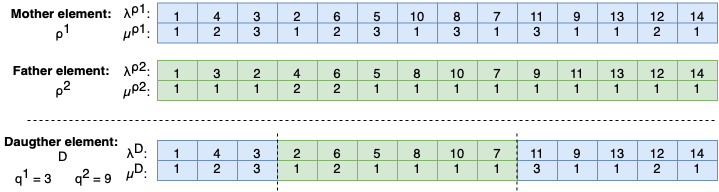
\includegraphics[width=0.93\textwidth]{assets/img/04_Umsetzung/TwoPointCrossover.drawio.png}
    }
    \caption{Beispiel des Two-Point Crossover für das MRCPSP} 
    \label{img:twopointcrossover}
    \source{Eigene Darstellung}
\end{figure}


\subsubsection*{Umsetzung des Mutation Operator}

Der implementierte Mutation Operator soll innerhalb der Aktivitäts- und Moduslisten von Nachfahren $\lambda$ leichte Änderungen realisieren. Tupels von austauschbaren Aktivitäten werden hierbei jeweils mit einer Wahrscheinlichkeit von $p_{mutation} = \sigma$ miteinander vertauscht. Mit der selben Wahrscheinlichkeit $\sigma$ zudem wird für jede Aktivität erneut ein zufälliger Modus selektiert. \\

Die Wahl einer optimalen Mutationsrate $\sigma$ stellt eine Herausforderung dar. Die Rechenberg Regel modifiziert die Mutationsrate $\sigma$ in Abhängigkeit der Erfolgsrate einer Population. Bei einer Erfolgsrate von weniger als 1/5 wird die Rate erhöht, bei 1/5 bleibt die Mutationsrate gleich. Sofern die Erfolgsrate größer als 1/5 ist, wird die Mutationsrate erhöht. \cite[vgl.][S. 24 f.]{kramer_genetic_2017} \\

Eine abgewandelte Form der Rechenberg Regel wird für den umgesetzten Algorithmus verwendet. Für die Implementierung bezieht sich die Erfolgsrate auf die Verbesserung des besten Individuums. Eine Population, die das neue beste Individuum gemäß der Fitness beinhaltet, wird als erfolgreich angesehen. Die Mutationsrate $\sigma$ wird über die folgende Formel geändert:
\begin{align*}
    \sigma = \sigma * \exp^{0.05}(a - \tfrac{1}{5}) && \text{mit }a = \begin{cases}
    0 & \text{mit Erfolgsrate} < 1/5 \\ 
    1 & \text{mit Erfolgsrate} \geq 1/5 \\ 
    \end{cases}
\end{align*}

\subsubsection*{Umsetzung des Selection Operator}
Bei dem implementierten Algorithmus handelt es sich um ein $(\mu+\lambda)-GA$, wobei die Lebensdauer einer Lösung auf $\kappa$ Generationen beschränkt ist. Wenn somit ein Individuum über $\kappa$ Generationen in die kommenden Population ausgewählt wurde, so wird die Lösung nicht mehr in der kommenden Population selektiert werden können. Es gilt das Individuum zu selektieren, für welches der Wert der Fitnessfunktion $f(x)$ am geringsten ist. 

\subsubsection*{Umsetzung der Fitnessfunktion}
Die umgesetzte Fitnessfunktion $f(x)$ orientiert sich an den Definitionen und der Priorisierungen der Zielfunktionen aus Abschnitt \ref{sec:AuswahlMetaheuristischenAlgorithmen}. Dadurch resultiert eine weitaus stärkere Gewichtung der Projektdauer $C_{max}$ im Vergleich zur Robustheit $\Omega$. Die Fitnessfunktion $f(x)$ ist gemäß dieser Gewichtung über die folgende Formel definiert:
\begin{align*}
f(x) = C_{max}(x) - \dfrac{\Omega(x)}{100}
\end{align*}

